\documentclass[11pt]{article}

% --------------------
% Packages
% --------------------
\usepackage[margin=1in]{geometry}
\usepackage{amsmath, amssymb, amsfonts}
\usepackage{mathtools}
\usepackage{enumitem}
\usepackage{titlesec}
\usepackage{fancyhdr}
\usepackage[dvipsnames]{xcolor}
\usepackage[colorlinks=true,linkcolor=blue]{hyperref}
\usepackage{physics}
\usepackage{tikz}
\usetikzlibrary{positioning}
\usetikzlibrary{calc,angles,quotes}
\usepackage{cancel}
\usepackage{array}
\usepackage{tcolorbox}
\usepackage[useregional]{datetime2} % optional formatting
\usepackage[outline]{contour} % glow around text
\usetikzlibrary{patterns,snakes}
\usetikzlibrary{arrows.meta} % for arrow size

\colorlet{xcol}{blue!70!black}
\colorlet{darkblue}{blue!40!black}
\colorlet{myred}{red!65!black}
\tikzstyle{mydashed}=[xcol,dashed,line width=0.25,dash pattern=on 2.2pt off 2.2pt]
\tikzstyle{axis}=[->,thick] %line width=0.6
\tikzstyle{ell}=[{Latex[length=3.3,width=2.2]}-{Latex[length=3.3,width=2.2]},line width=0.3]
\tikzstyle{dx}=[-{Latex[length=3.3,width=2.2]},darkblue,line width=0.3]
\tikzstyle{ground}=[preaction={fill,top color=black!10,bottom color=black!5,shading angle=20},
                    fill,pattern=north east lines,draw=none,minimum width=0.3,minimum height=0.6]
\tikzstyle{mass}=[line width=0.6,red!30!black,fill=red!40!black!10,rounded corners=1,
                  top color=red!40!black!20,bottom color=red!40!black!10,shading angle=20]
\tikzstyle{spring}=[line width=0.8,blue!7!black!80,snake=coil,segment amplitude=5,segment length=5,line cap=round]
\tikzset{>=latex} % for LaTeX arrow head
\tikzstyle{force}=[->,myred,very thick,line cap=round]
\def\tick#1#2{\draw[thick] (#1)++(#2:0.1) --++ (#2-180:0.2)}

% --------------------
% Page Style
% --------------------
\pagestyle{fancy}
\fancyhf{}
\fancyhead[L]{Physics II}
\fancyhead[R]{Lecture Notes}
\fancyfoot[C]{\thepage}

% --------------------
% Section Formatting
% --------------------
\titleformat{\section}
  {\normalfont\Large\bfseries}{Lecture \thesection}{1em}{}

\titleformat{\subsection}
  {\normalfont\large\bfseries}{\thesubsection}{1em}{}

\setlist[itemize]{noitemsep}

% --------------------
% Custom Commands
% --------------------
\newcommand{\R}{\mathbb{R}}
\newcommand{\mat}[1]{\begin{pmatrix} #1 \end{pmatrix}}
\newcommand{\changelink}[2]{\hyperref[#1]{#2}}

% Compact style: DD/MM/YY + 12-hour time
\newcommand{\compactdatetime}{%
  % Date: DD/MM/YY
  \the\day/\the\month/\the\numexpr\year-2000\relax\ %
  % Time: 12-hour
}
% --------------------
% Document Info
% --------------------
\title{\vspace{-2em}Physics II — Lecture Notes}
\author{Based on class notes by Jake Bobowski}
\date{Last updated: \compactdatetime}

% --------------------
% Document
% --------------------
\begin{document}

\maketitle
\vspace{-1em}
\noindent\text{Click on a section to jump there!}
\tableofcontents
\newpage

\begin{tcolorbox}[
  title={Recent Updates \hfill Last updated: \compactdatetime 2:20PM},
  colback=gray!5,
  colframe=black!40,
  boxrule=0.5pt,
  arc=4pt,
  fonttitle=\bfseries
]
\begin{itemize}
  \item \textbf{Jan 11}: Fixed graphics and small math errors: 
  \subitem\changelink{sec:lecture2.1-mass-on-spring}{Subsection 2.1 -- Mass on a Spring}
  \subitem\changelink{sec:lecture2.2-pendulum}{Subsection 2.2 -- Pendulum}
  \subitem\changelink{sec:aside2.2.1-rotational-motion}{Aside -- Rotational Motion}
  \subitem\changelink{sec:aside2.3.1-small-angle-approx}{Aside -- Small Angle Approximation}
  
  
  \item \textbf{Jan 10}: Added illustration to \changelink{sec:lecture2-rotational-motion}{Lecture 2 -- Concepts of Rotational Motion and General Oscillations}
  \subitem Added illustration of atom (Subsection 1.1.1)
  \subitem Added illustration of $\vec{F}$ and $\vec{E}$ (Subsection 1.1.2)
  
  
  \item \textbf{Jan 9}: Added content to Lecture 2:
  \subitem\changelink{sec:lecture2-rotational-motion}{Lecture 2 -- Concepts of Rotational Motion and General Oscillations}
  \subitem\changelink{sec:lecture2.1-mass-on-spring}{Subsection 2.1 -- Mass on a Spring}
  \subitem\changelink{sec:lecture2.2-pendulum}{Subsection 2.2 -- Pendulum}
  \subitem\changelink{sec:aside2.2.1-rotational-motion}{Aside -- Rotational Motion}
  \subitem\changelink{sec:aside2.3.1-small-angle-approx}{Aside -- Small Angle Approximation}
\end{itemize}
\end{tcolorbox}

% =====================================================
\newpage

\section{Electricity and Magnetism Introduction}
\subsection{The Electrostatic Force}
The electrostatic force is one of the forces that we experience continuously.

\subsubsection{The Atom}
All physical objects are made out of atoms. It contains:
\begin{enumerate}
    \item A positive core, which is the \textbf{nucleus}, and
    \item surrounded by a cloud of electrons. 
\end{enumerate}

\begin{center}
    \begin{tikzpicture}[scale=1.5]

% --- Electron cloud (very irregular boundary) ---
\draw[thick, blue]
  plot[smooth cycle, tension=0.6]
  coordinates {
    (2.4,0.3)
    (1.9,1.6)
    (0.7,2.3)
    (-0.9,2.0)
    (-2.0,1.1)
    (-2.4,0.0)
    (-2.1,-1.2)
    (-1.2,-2.2)
    (0.4,-2.4)
    (1.6,-1.9)
    (2.3,-0.9)
  };

% --- Many negative charges in the cloud ---
\foreach \x/\y in {
  1.5/0.7, 0.8/1.5, -0.4/1.7, -1.3/1.0,
  -1.8/0.2, -1.2/-0.8, -0.3/-1.6, 0.7/-1.8,
  1.6/-1.0, 1.9/-0.1, 0.2/0.6, -0.6/0.3
}{
  \node[blue] at (\x,\y) {$-$};
}

% --- Nucleus (denser, multiple pluses) ---
\draw[thick] (0,0) circle (0.18);

\foreach \x/\y in {
  0/0, 0.05/0.05, -0.05/-0.05, 0.06/-0.04
}{
  \node at (\x,\y) {\small $+$};
}

% --- Nucleus label ---
\draw[->] (0.35,0.25) -- (1.0,0.7)
  node[right] {$r_n \sim 10^{-15}\,\mathrm{m}$};

% --- Atomic radius label ---
\draw[->, blue] (-1.7,1.8) -- (-2.5,2.4)
  node[left, blue] {$r_a \sim 10^{-11}\,\mathrm{m}$};

\end{tikzpicture}
\end{center}

\vspace{1em}

\noindent For a typical atom like carbon, the nucleus' radius is around $3\times10^{-15}$m. On the other hand, the atom's radius is $\approx$ $7\times10^{-11}$m. The ratio of these two radii:
\begin{align*}
    \frac{r_{\text{atom}}}{r_{\text{nucleus}}} = \frac{10^{-11}}{10^{-15}} = 10^4
\end{align*}

\noindent Therefore, the atom is mostly "empty" space with the vast majority of its mass in a tiny core. To get a sense of this: 

\[
\begin{aligned}
\frac{d_{\text{moon}}}{r_{\text{earth}}} \approx 60
\end{aligned}
\qquad
\frac{d_{\text{Sun-Earth}}}{r_{\text{Sun}}} \approx 215
\]

\subsubsection{Electrostatic Repulsion}
When one touches a table, or any other object, one does not physically come in contact with anything. What on experiences is the electric repulsion between $e^-$ (electrons) in the atoms of one's hand and those of the table.

\vspace{0.5em}

\noindent Then how does one experience contact forces such as the normal force? Just as the gravitational force does not require contact and acts at a distance via a gravitational field, electric charges establish electric fields that can exert forces on other charges. 

\vspace{1.5em}

\noindent\textbf{Core Concept.} The electrostatic force is along the direction of the electric field, denoted by $\vec{E}$, which is a vector. 
\begin{center}
    \begin{tikzpicture}[scale=2.5]

% Charges
\node at (-1,-0.25) {$e^{-}$};
\node at (2,0.25) {$p^{+}$};

\fill (-1,0) circle (1.2pt);
\fill (2,0) circle (1.2pt);

% Separation
\draw[dashed] (-1,0) -- (1,0);

% Electric field at proton (longer)
\draw[->, thick, blue]
  (2,0) -- (0.8,0)
  node[midway, above] {$\vec{E}$};

% Force on proton (shorter)
\draw[->, thick, green!70!black]
  (2,0) -- (1.3,0)
  node[midway, below] {$\vec{F}$};

\end{tikzpicture}
\end{center}

\subsubsection{Magnets and Electricity}

\textbf{Core Concept.} The magnetic force is perpendicular to both:
\begin{enumerate}
    \item the direction of $\vec{B}$,
    \item and the direction of the charge's velocity, $\vec{v}$.
\end{enumerate}

\vspace{0.5em}

\begin{center}
    \begin{tikzpicture}[scale=2.5]
        \draw[->, thick] (0,0) -- (1.2,0)
    node[right] (v) {$\vec{v}$};

  % Into-the-page vector
  \node at (0,0) {$\otimes$};
  \node[above right=1pt] {$\vec{B}$};

  % Force vectors
  \draw[->, thick] (0,0) -- (0,1.2) node[above] {$\vec{F_{b}}$};
  \draw[->, thick] (0,0) -- (1.2,0) node[right] {$\vec{v}$};

\end{tikzpicture}
\end{center}

\noindent In this picture, we can conclude that $\vec{F_b} \perp \vec{B} \perp \vec{v}$. This is a special case of circular motion as $\vec{F_b} \perp \vec{v}$.


% =====================================================
\section{Concepts of Rotational Motion and General Oscillations}
\label{sec:lecture2-rotational-motion}

\subsection{Mass on a Spring}
\label{sec:lecture2.1-mass-on-spring}

\noindent Here is a mass on a spring in its \textbf{equilibrium position}.

\begin{center}
    % HORIZONTAL spring - axis, rest position
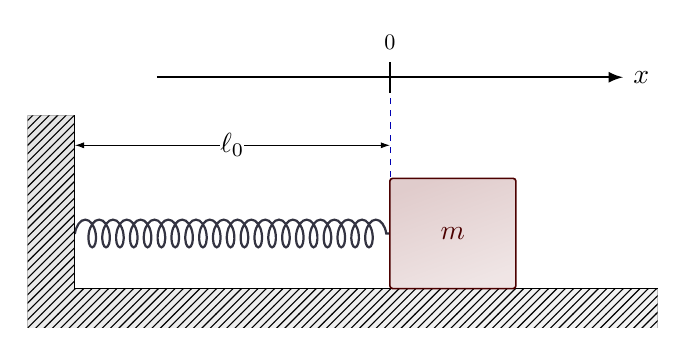
\begin{tikzpicture}[scale = 2]
  \def\H{1.1}  % wall height
  \def\T{0.3}  % wall thickness
  \def\W{3.7}  % ground length
  \def\D{0.25} % ground depth
  \def\h{0.7}  % mass height
  \def\w{0.8}  % mass width
  \def\x{2.0}  % mass x position
  \def\y{1.22*\H} % x axis y position
  
  % AXIS
  \draw[mydashed] (\x,0.9*\h) --++ (0,\y-0.9*\h);
  \draw[axis] (\x-0.4*\W,\y) -- (\x+0.4*\W,\y) node[right] {$x$};
  \tick{\x,\y}{-90} node[scale=0.8,above=0.05] {$0$};
  \draw[ell] (0,1.3*\h) --++ (\x,0) node[midway,fill=white,inner sep=0] {$\ell_0$};
  
  % SPRING & MASS
  \draw[spring] (0,\h/2) --++ (\x,0);
  \draw[ground] (0,0) |-++ (-\T,\H) |-++ (\T+\W,-\H-\D) -- (\W,0) -- cycle;
  \draw (0,\H) -- (0,0) -- (\W,0);
  \draw[mass] (\x,0) rectangle++ (\w,\h) node[midway] {$m$};
  
\end{tikzpicture}
\end{center}


\noindent Here is its \textbf{extended} position:

\begin{center}
    % HORIZONTAL spring - axis, extended
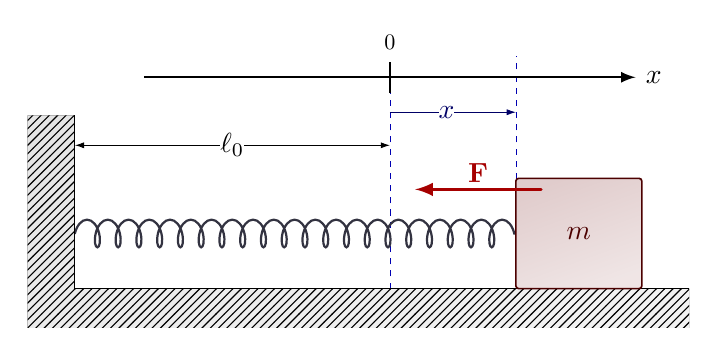
\begin{tikzpicture}[scale = 2]
  \def\H{1.1}  % wall height
  \def\T{0.3}  % wall thickness
  \def\W{3.9}  % ground length
  \def\D{0.25} % ground depth
  \def\h{0.7}  % mass height
  \def\w{0.8}  % mass width
  \def\x{2.0}  % mass x position
  \def\dx{0.8} % extension
  \def\y{1.22*\H} % x axis y position
  \def\F{0.8}  % force
  
  % AXIS
  \draw[mydashed] (\x,0) --++ (0,\y) (\x+\dx,0) --++ (0,1.1*\y);
  \draw[axis] (\x-0.4*\W,\y) -- (\x+0.4*\W,\y) node[right] {$x$};
  \tick{\x,\y}{-90} node[scale=0.8,above=0.05] {$0$};
  \draw[ell] (0,1.3*\h) --++ (\x,0) node[midway,fill=white,inner sep=0] {$\ell_0$};
  \draw[dx] (\x,1.6*\h) --++ (\dx,0) node[pos=0.45,fill=white,inner sep=0] {$x$};
  
  % SPRING & MASS
  \draw[spring,segment length=7.5] (0,\h/2) --++ (\x+\dx,0);
  \draw[ground] (0,0) |-++ (-\T,\H) |-++ (\T+\W,-\H-\D) -- (\W,0) -- cycle;
  \draw (0,\H) -- (0,0) -- (\W,0);
  \draw[mass] (\x+\dx,0) rectangle++ (\w,\h) node[midway] {$m$};
  \draw[force] (\x+\dx+0.2*\w,0.9*\h) --++ (-\F,0) node[midway,right=1,above=-0.05] {$\vb{F}$};
  
\end{tikzpicture}
\end{center}

\vspace{1em}

\noindent Here is its \textbf{compressed} position:

\begin{center}
    % HORIZONTAL spring - axis, compressed
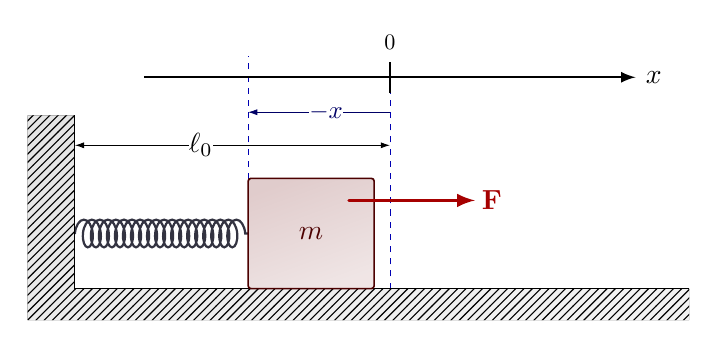
\begin{tikzpicture}[scale = 2]
  \def\H{1.1} % wall height
  \def\T{0.3} % wall thickness
  \def\W{3.9} % ground length
  \def\D{0.2} % ground depth
  \def\h{0.7} % mass height
  \def\w{0.8} % mass width
  \def\x{2.0} % mass x position
  \def\dx{0.9} % extension
  \def\y{1.22*\H} % x axis y position
  \def\F{0.8} % force
  
  % AXIS
  \draw[mydashed] (\x,0) --++ (0,\y) (\x-\dx,0) --++ (0,1.1*\y);
  \draw[axis] (\x-0.4*\W,\y) -- (\x+0.4*\W,\y) node[right] {$x$};
  \tick{\x,\y}{-90} node[scale=0.8,above=0.05] {$0$};
  \draw[ell] (0,1.3*\h) --++ (\x,0) node[pos=0.4,fill=white,inner sep=0] {$\ell_0$};
  \draw[dx] (\x,1.6*\h) --++ (-\dx,0)
    node[pos=0.45,fill=white,inner sep=0,scale=0.9] {$-x$};
  
  % SPRING & MASS
  \draw[spring,segment length=2.9] (0,\h/2) --++ (\x-\dx,0);
  \draw[ground] (0,0) |-++ (-\T,\H) |-++ (\T+\W,-\H-\D) -- (\W,0) -- cycle;
  \draw (0,\H) -- (0,0) -- (\W,0);
  \draw[mass] (\x-\dx,0) rectangle++ (\w,\h) node[midway] {$m$};
  \draw[force] (\x-\dx+0.8*\w,0.8*\h) --++ (\F,0) node[below=0,right=-0.05] {$\vb{F}$};
  
\end{tikzpicture}
\end{center}


\noindent The spring force on a mass $m$ is given through the formula $F_s = -kx$. This is classified as a restoring force.

\vspace{1em}

\noindent Newton's 2nd Law states that $F = ma$. Recall that:
\begin{align*}
    a = \dfrac{dv}{dt}\ = \dfrac{d}{dt}\left(\dfrac{dx}{dt}\right) = \dfrac{d^2x}{dt^2} \\
\end{align*}
\noindent And so substituting in for $a$: 

\begin{equation}
    m\dfrac{d^2x}{dt^2} = -kx
\end{equation}

\noindent To find $x(t)$, or the time evolution of $x$, we need a function that after taking two derivatives, returns the original function with a negative sign. Let us try the function $A\cos{(\omega t})$, where $A$ is the amplitude/initial displacement, and $\omega$ is the angular frequency. As a consequence of the chain rule: 

\begin{align*}
    \vec{v} = \dfrac{dx}{dt} = -\omega A\cos{(\omega t)} 
\end{align*}

Differentiating the second time:

\begin{equation}
   \vec{a} = \dfrac{d\vec{v}}{dt} = -\omega^{2} A\cos{(\omega t)}
\end{equation}

\begin{align*}
    \therefore \text{ We can say } A\cos{(\omega t) = x \Rightarrow \dfrac{d^2 x}{dt^2}= -\omega^{2} x}.
\end{align*}

Substituting (2) into (1):
\begin{align*}
    m(-\omega^{2}x)&=-kx \\
    m(\cancel{-}\omega^{2}\cancel{x})&=\cancel{-}k\cancel{x} \\
    \therefore w^2 = \frac{k}{m} \text{ or } w &= \sqrt{\frac{k}{m}}
\end{align*}

where $\sqrt{\frac{k}{m}}$ is the angular frequency of a mass on a spring.

\vspace{1em}

Recall that angular frequency, $\omega$, is $2\pi f$, where $f$ is the frequency or cycles/second. 
\begin{align*}
    \therefore \omega = 2 \pi f \\
    \text{ where } f= \frac{1}{T}.
\end{align*}

So, 
\begin{align*}
    T = 2\pi\sqrt{\frac{m}{k}}
\end{align*}

Notice $T$ of the motion is independent of the amplitude. 

% =====================================================

\subsection{Pendulum}
\label{sec:lecture2.2-pendulum}
Let us try to relate the problem of an oscillating pendulum to the mass on a spring.

\begin{center}
    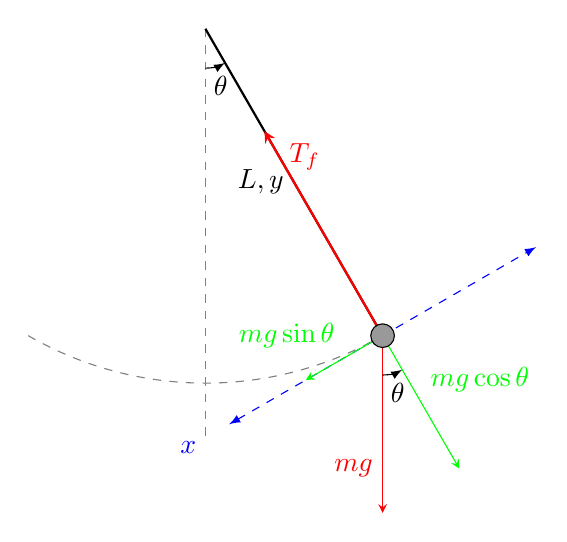
\begin{tikzpicture}[scale = 1.5]
    % save length of g-vector and theta to macros
    \pgfmathsetmacro{\Gvec}{1.5}
    \pgfmathsetmacro{\myAngle}{30}
    \pgfmathsetmacro{\pendulumLength}{3}
    
    % calculate lengths of vector components
    \pgfmathsetmacro{\Gcos}{\Gvec*cos(\myAngle)}
    \pgfmathsetmacro{\Gsin}{\Gvec*sin(\myAngle)}

    \coordinate (centro) at (0,0);
    \draw[dashed,gray,-] (centro) -- ++ (0,-3.5) node (mary) [black,below]{$ $};
    
    % 1. Dotted circular arc path
    \draw[dashed, gray] (270-\myAngle:\pendulumLength) arc (270-\myAngle:270+\myAngle:\pendulumLength);

    % Pendulum Arm (y-axis direction)
    \draw[thick] (centro) -- ++(270+\myAngle:\pendulumLength) coordinate (bob)
      node[midway, left] {$L,y$};
    
    % Top Angle
    \pic [draw, ->, "$\theta$", angle eccentricity=1.5] {angle = mary--centro--bob};

    % 2. Extended Tangent x-axis (Dotted)
    % This draws a line through the bob, perpendicular to the string
    \draw[dashed, blue, <->] ($(bob)!1.5cm!90:(centro)$) -- ($(bob)!1.5cm!-90:(centro)$);
    \node[blue] at ($(bob)!1.9cm!90:(centro)$) {$x$};

    % 3. Tension Force (T_f) - BLUE
    \draw [red,-stealth, thick] (bob) -- ($(bob)!2.0cm!(centro)$) 
      node[very near end, right] {$T_f$};

    % Gravity Components
    % Radial component pointing away from centro (mg cos theta)
    \draw [green, -stealth] (bob) -- ($(bob)!-\Gcos cm!(centro)$)
      coordinate (gcos)
      node[midway,above right] {$mg\cos\theta$};
      
    % Tangential component (mg sin theta)
    \draw [green, -stealth] (bob) -- ($(bob)!\Gsin cm!90:(centro)$)
      coordinate (gsin)
      node[midway,above left] {$mg\sin\theta$};
      
    % Gravity Vector
    \draw [red, -stealth] (bob) -- ++(0,-\Gvec)
      coordinate (g)
      node[near end,left] {$mg$};
      
    % Bottom Angle
    \pic [draw, ->, "$\theta$", angle eccentricity=1.5] {angle = g--bob--gcos};
    
    % The Bob
    \filldraw [fill=black!40,draw=black] (bob) circle[radius=0.1];
\end{tikzpicture}
\end{center}

\noindent We have decomposed our forces into components along the $x$ and $y$ axes. We will analyze the net force along the $x$ and $y$ directions. In the $y$-direction:
\begin{align*}
    F_y = ma_y = T_f -mg\cos\theta = 0
\end{align*}

We have no up and down motion so this is equal to 0,
\begin{align*}
    \therefore T_f = mg\cos\theta
\end{align*}

In the x-direction: 
\begin{align*}
    F_x = ma_x = mg\sin\theta \\
    F_x = \cancel{m}a_x = \cancel{m}g\sin\theta
\end{align*}
\begin{equation}
    \therefore a_x = -g\sin\theta
\end{equation}

\noindent Equation (3) is not quite the same as the mass on the spring. We can make some manipulations to make it similar. 

% =====================================================

\subsubsection{Aside: Rotational Motion}
\label{sec:aside2.2.1-rotational-motion}
\vspace{1em}

\[
\begin{tabular}{m{5cm} @{\hspace{1cm}} m{5cm}} % '@' adds specific spacing between columns
    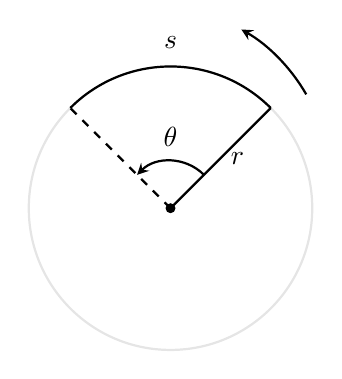
\begin{tikzpicture}[>=stealth, thick, scale=1.5]
        % 1. Draw the full circle in light gray
        \draw[gray!20] (0,0) circle (1.2cm);
        
        % 2. Draw the 90-degree "Pizza Slice" pointing up
        \coordinate (O) at (0,0);
        \draw (O) -- (45:1.2cm) node[midway, right] {$r$};
        \draw[dashed] (O) -- (135:1.2cm) node[midway, left]{};
        \draw[thick] (45:1.2cm) arc (45:135:1.2cm);
        
        % 3. Label for the arc 's'
        \node at (90:1.4cm) {$s$};
        
        % 4. Angle label theta inside
        \draw [->] (45:0.4cm) arc (45:135:0.4cm);
        \node at (90:0.6cm) {$\theta$};

        % 5. External rotation arrow
        \draw[->] (40:1.5cm) arc (30:60:1.5cm);
        
        % Origin point
        \fill (O) circle (1.2pt);
    \end{tikzpicture}
    & 
    % Wrap the table in a minipage aligned to the top [t]
    \begin{minipage}[t]{4cm}
        \vspace{-1cm} % Adjust this value to move the text up or down exactly where you want it
        \begin{tabular}{l}
            Circumference is $C = 2 \pi r$, \\
            the angle for a round trip on the \\
            circumference.
        \end{tabular}
    \end{minipage}
\end{tabular}
\]

\vspace{1em}

\[
\begin{tabular}{m{5cm} @{\hspace{1cm}} m{5cm}} % '@' adds specific spacing between columns
    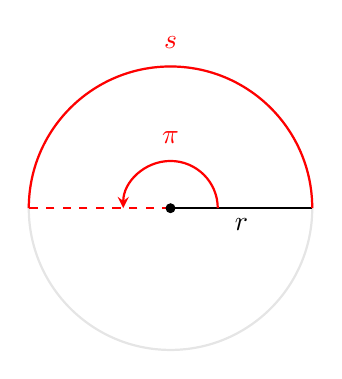
\begin{tikzpicture}[>=stealth, thick, scale=1.5]
    % 1. Draw the full circle in light gray
    \draw[gray!20] (0,0) circle (1.2cm);
    
    % 2. Define Center
    \coordinate (O) at (0,0);
    
    % 3. Draw the horizontal radius (Solid, to the right)
    % 0:1.2cm means 0 degrees (horizontal)
    \draw (O) -- (0:1.2cm) node[midway, below] {$r$};

    \node[red] at (90:1.4cm) {$s$};
    
    % 4. Draw the opposite radius (Dashed, to the left)
    % 180:1.2cm is the far left
    \draw[red, dashed] (O) -- (180:1.2cm);
    
    \draw[thick, red] (0:1.2cm) arc (0:180:1.2cm);

    % 5. Draw the angle arrow (theta = pi)
    % It starts at 0 degrees and sweeps to 180 degrees
    \draw [red, ->] (0.4,0) arc (0:180:0.4cm);
    \node[red] at (90:0.6cm) {$\pi$};

    % Origin point
    \fill (O) circle (1.2pt);
\end{tikzpicture}
    & 
    % Wrap the table in a minipage aligned to the top [t]
    \begin{minipage}[t]{4cm}
        \vspace{-1cm} % Adjust this value to move the text up or down exactly where you want it
        \begin{tabular}{l}
            Arclength is $S = \pi r$, \\
            the area travelled along our arc.
        \end{tabular}
    \end{minipage}
\end{tabular}
\]

\[
\begin{tabular}{m{5cm} @{\hspace{1cm}} m{5cm}}
    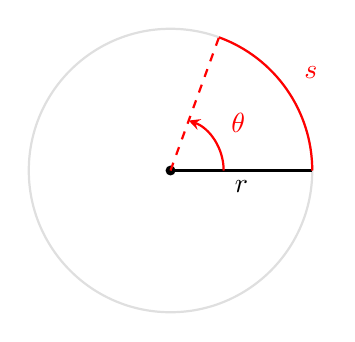
\begin{tikzpicture}[>=stealth, thick, scale=1.5]

        % Circle
        \draw[gray!25] (0,0) circle (1.2cm);

        % Center
        \coordinate (O) at (0,0);
        \fill (O) circle (1.2pt);

        % Radius lines
        \draw (O) -- (0:1.2cm) node[midway, below] {$r$};
        \draw[red, dashed] (O) -- (70:1.2cm);

        % Arc corresponding to angle theta
        \draw[thick, red] (0:1.2cm) arc (0:70:1.2cm);

        % Arc label s
        \node[red] at (35:1.45cm) {$s$};

        % Angle theta (radians)
        \draw[->, red] (0:0.45cm) arc (0:70:0.45cm);
        \node[red] at (35:0.7cm) {$\theta$};

    \end{tikzpicture}
    &
    \begin{minipage}[t]{4cm}
        \vspace{-1cm}
        \begin{tabular}{l}
            Arclength is $S = \theta r$, the \\
            angle traveled in radians.
        \end{tabular}
    \end{minipage}
\end{tabular}
\]




\vspace{0.5em}

% =====================================================


\subsection{Pendulum Continued}
What about the speed?
\begin{align*}
    \vec{v} = \dfrac{ds}{dt} = \dfrac{d}{dt}(r\theta)
\end{align*}

For circular motion, $r$ is constant so:
\begin{align*}
    \vec{v} = r\cdot\dfrac{d\theta}{dt}
\end{align*}

Finally, 
\begin{equation}
    a = \dfrac{d\vec{v}}{dt} = \dfrac{d}{dt} \left(r\dfrac{d\theta}{dt}\right) = r\dfrac{d^2 
    \theta}{dt^2}
\end{equation}

\vspace{1em}

Use Equation (4) in (3). For our pendulum, $r = L$.
\begin{align*}
    a_x = -g\sin\theta \\
    L\dfrac{d^2 
    \theta}{dt^2} = -g\sin\theta
\end{align*}

or

\begin{align*}
    \dfrac{d^2 \theta}{dt^2} = -\frac{g}{L}\sin\theta
\end{align*}

where $\theta$ is the angular position. Going back to our mass on a spring,
\begin{align*}
    \dfrac{d^2 x}{dt^2} = -\frac{k}{m}x
\end{align*}

\noindent where $x$ is the linear position of a mass on a spring. These are similar but not identical. We have $\sin\theta$ instead of $\theta$. We will consider the \textbf{small angle approximation.}

% =====================================================

\subsubsection{Aside: Small Angle Approximation}
\label{sec:aside2.3.1-small-angle-approx}


\begin{center}
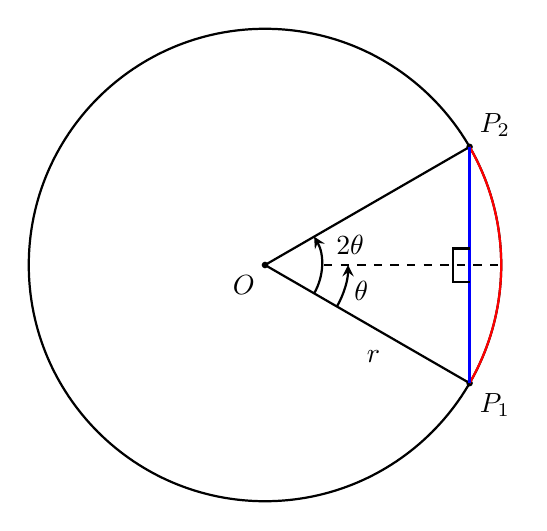
\begin{tikzpicture}[scale=3, thick]

% Circle
\draw (0,0) circle (1);

% Center and reference point
\coordinate (O) at (0,0);
\coordinate (A) at (1,0);
\fill (O) circle (0.4pt) node[below left] {$O$};

% Points on circle
\coordinate (P1) at ({cos(-30)},{sin(-30)});
\coordinate (P2) at ({cos(30)},{sin(30)});

\fill (P1) circle (0.4pt) node[below right] {$P_1$};
\fill (P2) circle (0.4pt) node[above right] {$P_2$};

% Horizontal dashed reference line
\draw[dashed] (0.25,0) -- (1,0);

% Radii
\draw (O) -- (P1);
\draw (O) -- (P2);

% Radius label
\node at (-40:0.6) {$r$};

% Arc (s)
\draw[thick, red] (30:1) arc (30:-30:1);

% Chord
\draw[blue] (P1) -- (P2);

% Foot of perpendicular (EXACT)
\coordinate (F) at ({cos(30)},0);

% Right angle marker (visible)
\pic [draw, angle radius=6pt] {right angle = P2--F--O};
\pic [draw, angle radius=6pt] {right angle = P1--F--O};

% Angle arcs
\pic [draw, -stealth, "$2\theta$", angle radius=20.5, angle eccentricity=1.5, above]
    {angle = P1--O--P2};

\pic [draw, -stealth, "$\theta$", angle radius=30, angle eccentricity=1.2]
    {angle = P1--O--A};

\end{tikzpicture}
\end{center}

\vspace{1em}
\noindent The distance from $P_1$ to $O$, is mathematically expressed as: 
\begin{align*}
    d = r\sin\theta
\end{align*}

\noindent And so it follows that the distance from $P_1$ to $P_2$, which we will denote by distance $d$:
\begin{align*}
    d = 2r\sin\theta
\end{align*}

\vspace{1.5em}

\noindent The arc length between $P_1$ and $P_2$ has the length of
\begin{align*}
    s = 2r\theta
\end{align*}
by the definition of the radian measure.

\vspace{1.5em}
\noindent Comparing $s$ and $d$, it's clear that $s>d$:
\begin{align*}
    s = 2r\theta > 2r\sin\theta \\
    s = \cancel{2r}\theta > \cancel{2r}\sin\theta \\
\end{align*}

\noindent So,
\begin{align*}
     \therefore \theta > \sin\theta
\end{align*}

\end{document}
